\chapter{Giới thiệu}
\label{ch:gioi-thieu}

\section{Bối cảnh và vấn đề nghiên cứu}
\label{sec:boi-canh}

Rối loạn trầm cảm (Major Depressive Disorder -- MDD) là một trong những nguyên nhân hàng đầu gây suy giảm chất lượng cuộc sống và gia tăng gánh nặng y tế trên quy mô toàn cầu \cite{pratt1991discriminant}. Theo Tổ chức Y tế Thế giới (WHO), hơn 300 triệu người thuộc mọi lứa tuổi đang phải đối mặt với các mức độ trầm cảm khác nhau. Không chỉ gây ảnh hưởng tiêu cực đến sức khỏe tinh thần, năng suất làm việc và gắn kết xã hội, trầm cảm mức độ nặng còn là căn nguyên trực tiếp dẫn đến hàng trăm nghìn ca tự tử mỗi năm. Đáng lo ngại hơn, phần lớn những người có triệu chứng trầm cảm ở giai đoạn khởi phát hoặc mức độ nhẹ thường không nhận biết được tình trạng của bản thân, hoặc e ngại rào cản tâm lý xã hội (stigma), dẫn đến việc chậm trễ trong việc tiếp cận các dịch vụ chăm sóc và can thiệp y tế kịp thời.

Trong thực hành lâm sàng và các nghiên cứu dịch tễ học hiện nay, công cụ tiêu chuẩn được sử dụng rộng rãi nhất để sàng lọc và lượng giá mức độ triệu chứng trầm cảm là Thang đo Sức khỏe Bệnh nhân 9 mục (Patient Health Questionnaire-9 -- PHQ-9) do Kroenke và cộng sự phát triển \cite{kroenke2001phq, spitzer1999validation}. PHQ-9 bao gồm 9 câu hỏi tự điền tương ứng với 9 tiêu chuẩn chẩn đoán trầm cảm trong Sổ tay Chẩn đoán và Thống kê Rối loạn Tâm thần (DSM-IV). Mỗi câu hỏi được tính điểm từ 0 đến 3, tạo nên một thang điểm liên tục dao động từ 0 đến 27 điểm. Dựa vào tổng điểm số, y văn chia mức độ nghiêm trọng thành năm bậc lâm sàng rõ rệt: Tối thiểu (Minimal, 0--4 điểm), Nhẹ (Mild, 5--9 điểm), Vừa (Moderate, 10--14 điểm), Nặng vừa (Moderately severe, 15--19 điểm) và Rất nặng (Severe, 20--27 điểm).

Mặc dù PHQ-9 có giá trị sàng lọc cao, phương pháp này vẫn tồn tại những hạn chế cố hữu xuất phát từ bản chất tự báo cáo (self-reported questionnaire). Người tham gia khảo sát có thể phóng đại hoặc che giấu triệu chứng do các yếu tố tâm lý chủ quan, định kiến xã hội hoặc sự thiếu nhất quán trong việc tự nhận thức cảm xúc. Do đó, việc khai thác các chỉ số đo lường khách quan từ kiểm tra sức khỏe thể chất định kỳ và xét nghiệm cận lâm sàng nhằm hỗ trợ lượng giá mức độ triệu chứng trầm cảm là một hướng nghiên cứu có ý nghĩa thực tiễn to lớn trong y tế dự phòng và chăm sóc sức khỏe ban đầu.

Các cuộc điều tra sức khỏe quy mô quốc gia, tiêu biểu là Khảo sát Kiểm tra Sức khỏe và Dinh dưỡng Quốc gia Hoa Kỳ (National Health and Nutrition Examination Survey -- NHANES) do Trung tâm Thống kê Y tế Quốc gia (NCHS) thuộc CDC thực hiện định kỳ hai năm một lần \cite{cdc2014nhanes, cdc2016nhanes}, cung cấp một nguồn dữ liệu dạng bảng (tabular health data) phong phú. NHANES kết hợp phỏng vấn dịch tễ, thăm khám thể lực chi tiết và các xét nghiệm sinh hóa máu chuẩn hóa. Nhiều nghiên cứu y sinh học gần đây đã chỉ ra mối liên hệ gián tiếp giữa trầm cảm và các rối loạn chuyển hóa toàn thân, bao gồm phản ứng viêm mãn tính thể nhẹ, rối loạn lipid máu, sự dao động của huyết áp và chỉ số khối cơ thể (BMI).

Học máy (Machine Learning -- ML) sở hữu tiềm năng mạnh mẽ trong việc khai phá các mối quan hệ phi tuyến tính phức tạp giữa các chỉ số sinh lý đa chiều để dự đoán nguy cơ sức khỏe. Tuy nhiên, khi áp dụng Machine Learning vào bài toán dự đoán mức độ triệu chứng trầm cảm trên dữ liệu khảo sát cộng đồng dạng bảng như NHANES, các phương pháp tiếp cận truyền thống phải đối mặt với ba rào cản kỹ thuật nghiêm trọng:
\begin{enumerate}
    \item \textbf{Mất cân bằng lớp cực đoan (Severe Class Imbalance):} Trong quần thể dân cư nói chung, phần lớn người tham gia khảo sát không có hoặc chỉ có triệu chứng tối thiểu ($C_0$, chiếm 74--76\%), trong khi số lượng đối tượng có triệu chứng nặng ($C_4$) chỉ chiếm một tỷ lệ rất nhỏ (khoảng 1.0--1.3\%). Sự chênh lệch này khiến các mô hình học máy thông thường có xu hướng dự đoán toàn bộ về lớp đa số để đạt độ chính xác bề nổi (Accuracy) rất cao nhưng hoàn toàn thất bại trong việc nhận diện các ca bệnh thực tế.
    \item \textbf{Sự chồng lấn đặc trưng sinh lý cao (High Feature Overlap):} Khác với các bệnh lý thực thể có chỉ dấu sinh học đặc hiệu, các chỉ số sinh lý ngoại vi giữa người khỏe mạnh và người có triệu chứng trầm cảm nhẹ có độ phân tán và chồng lấn rất lớn. Các ranh giới phân tách trong không gian đặc trưng trở nên mờ nhạt, khiến các bộ phân loại phẳng truyền thống dễ nhầm lẫn giữa các mức độ kế cận.
    \item \textbf{Sự suy giảm hiệu năng theo độ chi tiết nhãn (Granularity Degradation):} Đa số các công trình trước đây chỉ dừng lại ở bài toán phân loại nhị phân ($T_2$: Có triệu chứng vs Không có triệu chứng). Khi bài toán được mở rộng sang phân loại đa mức độ ($T_3, T_4, T_5$) nhằm đáp ứng nhu cầu phân tầng rủi ro lâm sàng chi tiết, hiệu năng của các mô hình học máy bị suy giảm đột ngột và chưa có lời giải thỏa đáng.
\end{enumerate}

Xuất phát từ các thách thức trên, đề tài \textbf{“Nghiên cứu khung học máy cho dự đoán mức độ triệu chứng trầm cảm từ dữ liệu sinh lý”} được triển khai nhằm xây dựng và đánh giá toàn diện framework mang tên \textbf{DepSev-ML} (Depression Severity Machine Learning). Cần lưu ý rằng, nghiên cứu này không hướng tới việc thay thế bảng câu hỏi PHQ-9 hay đưa ra chẩn đoán lâm sàng tự động thay thế bác sĩ chuyên khoa tâm thần, mà tập trung vào việc nghiên cứu giới hạn dự đoán của các đặc trưng sinh lý dạng bảng và đề xuất các giải pháp kiến trúc học máy phù hợp nhằm nâng cao độ nhạy cho các nhóm bệnh nhân có nguy cơ cao.

\section{Phát biểu bài toán}
\label{sec:phat-bieu-bai-toan}

Bài toán nghiên cứu của DepSev-ML được phát biểu dưới dạng bài toán học có giám sát (Supervised Learning) trên dữ liệu dạng bảng.

Cho tập dữ liệu nghiên cứu gồm $N$ quan sát độc lập:
\begin{equation}
    \mathcal{D} = \{(\mathbf{x}_i, s_i)\}_{i=1}^N
\end{equation}
trong đó:
\begin{itemize}
    \item $\mathbf{x}_i \in \mathcal{X} \subseteq \mathbb{R}^d$ là vectơ đặc trưng $d$ chiều của đối tượng thứ $i$, bao gồm các biến số đo lường sinh lý (nhân trắc học, huyết áp), xét nghiệm cận lâm sàng (hóa sinh máu, huyết học), thông tin lối sống (hoạt động thể lực, giấc ngủ, hút thuốc, rượu bia) và nhân khẩu học.
    \item $s_i \in \{0, 1, 2, \dots, 27\}$ là tổng điểm PHQ-9 của đối tượng thứ $i$, được tính bằng tổng của 9 câu hỏi khảo sát thành phần:
    \begin{equation}
        s_i = \sum_{j=1}^9 \text{DPQ}_{ij}, \quad \text{với } \text{DPQ}_{ij} \in \{0, 1, 2, 3\}
    \end{equation}
\end{itemize}

Nhãn mục tiêu $y_i$ được sinh ra thông qua một hàm ánh xạ lượng giá $\Phi: \{0, \dots, 27\} \to \mathcal{Y}_K$, trong đó $\mathcal{Y}_K = \{0, 1, \dots, K-1\}$ là không gian đầu ra gồm $K$ mức độ nghiêm trọng rời rạc ($K \in \{2, 3, 4, 5\}$). Nghiên cứu định nghĩa bốn thiết lập độ phân giải mục tiêu:
\begin{itemize}
    \item \textbf{Thiết lập $T_2$ ($K=2$, Phân loại nhị phân):} $y_i = 0$ nếu $s_i \in [0, 4]$ (Tối thiểu); $y_i = 1$ nếu $s_i \in [5, 27]$ (Có triệu chứng).
    \item \textbf{Thiết lập $T_3$ ($K=3$, Ba nhóm gộp quy ước):} $y_i = 0$ nếu $s_i \in [0, 4]$ ($C_0$: Tối thiểu); $y_i = 1$ nếu $s_i \in [5, 9]$ ($C_1$: Nhẹ); $y_i = 2$ nếu $s_i \in [10, 27]$ ($C_2^+$: Nặng quy ước).
    \item \textbf{Thiết lập $T_4$ ($K=4$, Bốn mức độ):} $C_0$ ($0$--$4$), $C_1$ ($5$--$9$), $C_2$ ($10$--$14$), $C_3^+$ ($15$--$27$).
    \item \textbf{Thiết lập $T_5$ ($K=5$, Năm mức độ lâm sàng chuẩn PHQ-9):} $C_0$ (Minimal, $0$--$4$), $C_1$ (Mild, $5$--$9$), $C_2$ (Moderate, $10$--$14$), $C_3$ (Moderately severe, $15$--$19$), và $C_4$ (Severe, $20$--$27$).
\end{itemize}

Mục tiêu học máy là tìm kiếm một hàm dự đoán $f: \mathcal{X} \to \mathcal{Y}_K$ sao cho tối đa hóa độ đo hiệu năng trên toàn bộ các lớp. Do dữ liệu bị mất cân bằng lớp nghiêm trọng, hàm mục tiêu đánh giá chính của nghiên cứu không sử dụng Accuracy thông thường mà được xác định thông qua hai chỉ số chính:
\begin{equation}
    \text{Macro-F1} = \frac{1}{K} \sum_{k=0}^{K-1} \text{F1}_k = \frac{1}{K} \sum_{k=0}^{K-1} \frac{2 \cdot \text{Precision}_k \cdot \text{Recall}_k}{\text{Precision}_k + \text{Recall}_k}
\end{equation}
\begin{equation}
    \text{Balanced Accuracy} = \frac{1}{K} \sum_{k=0}^{K-1} \text{Recall}_k
\end{equation}

Sơ đồ tổng quan về bài toán và luồng xử lý của nghiên cứu được minh họa trong Hình \ref{fig:problem-formulation}.

\begin{figure}[htbp]{Sơ đồ tổng quan phát biểu bài toán và luồng xử lý của khung học máy DepSev-ML}
\centering
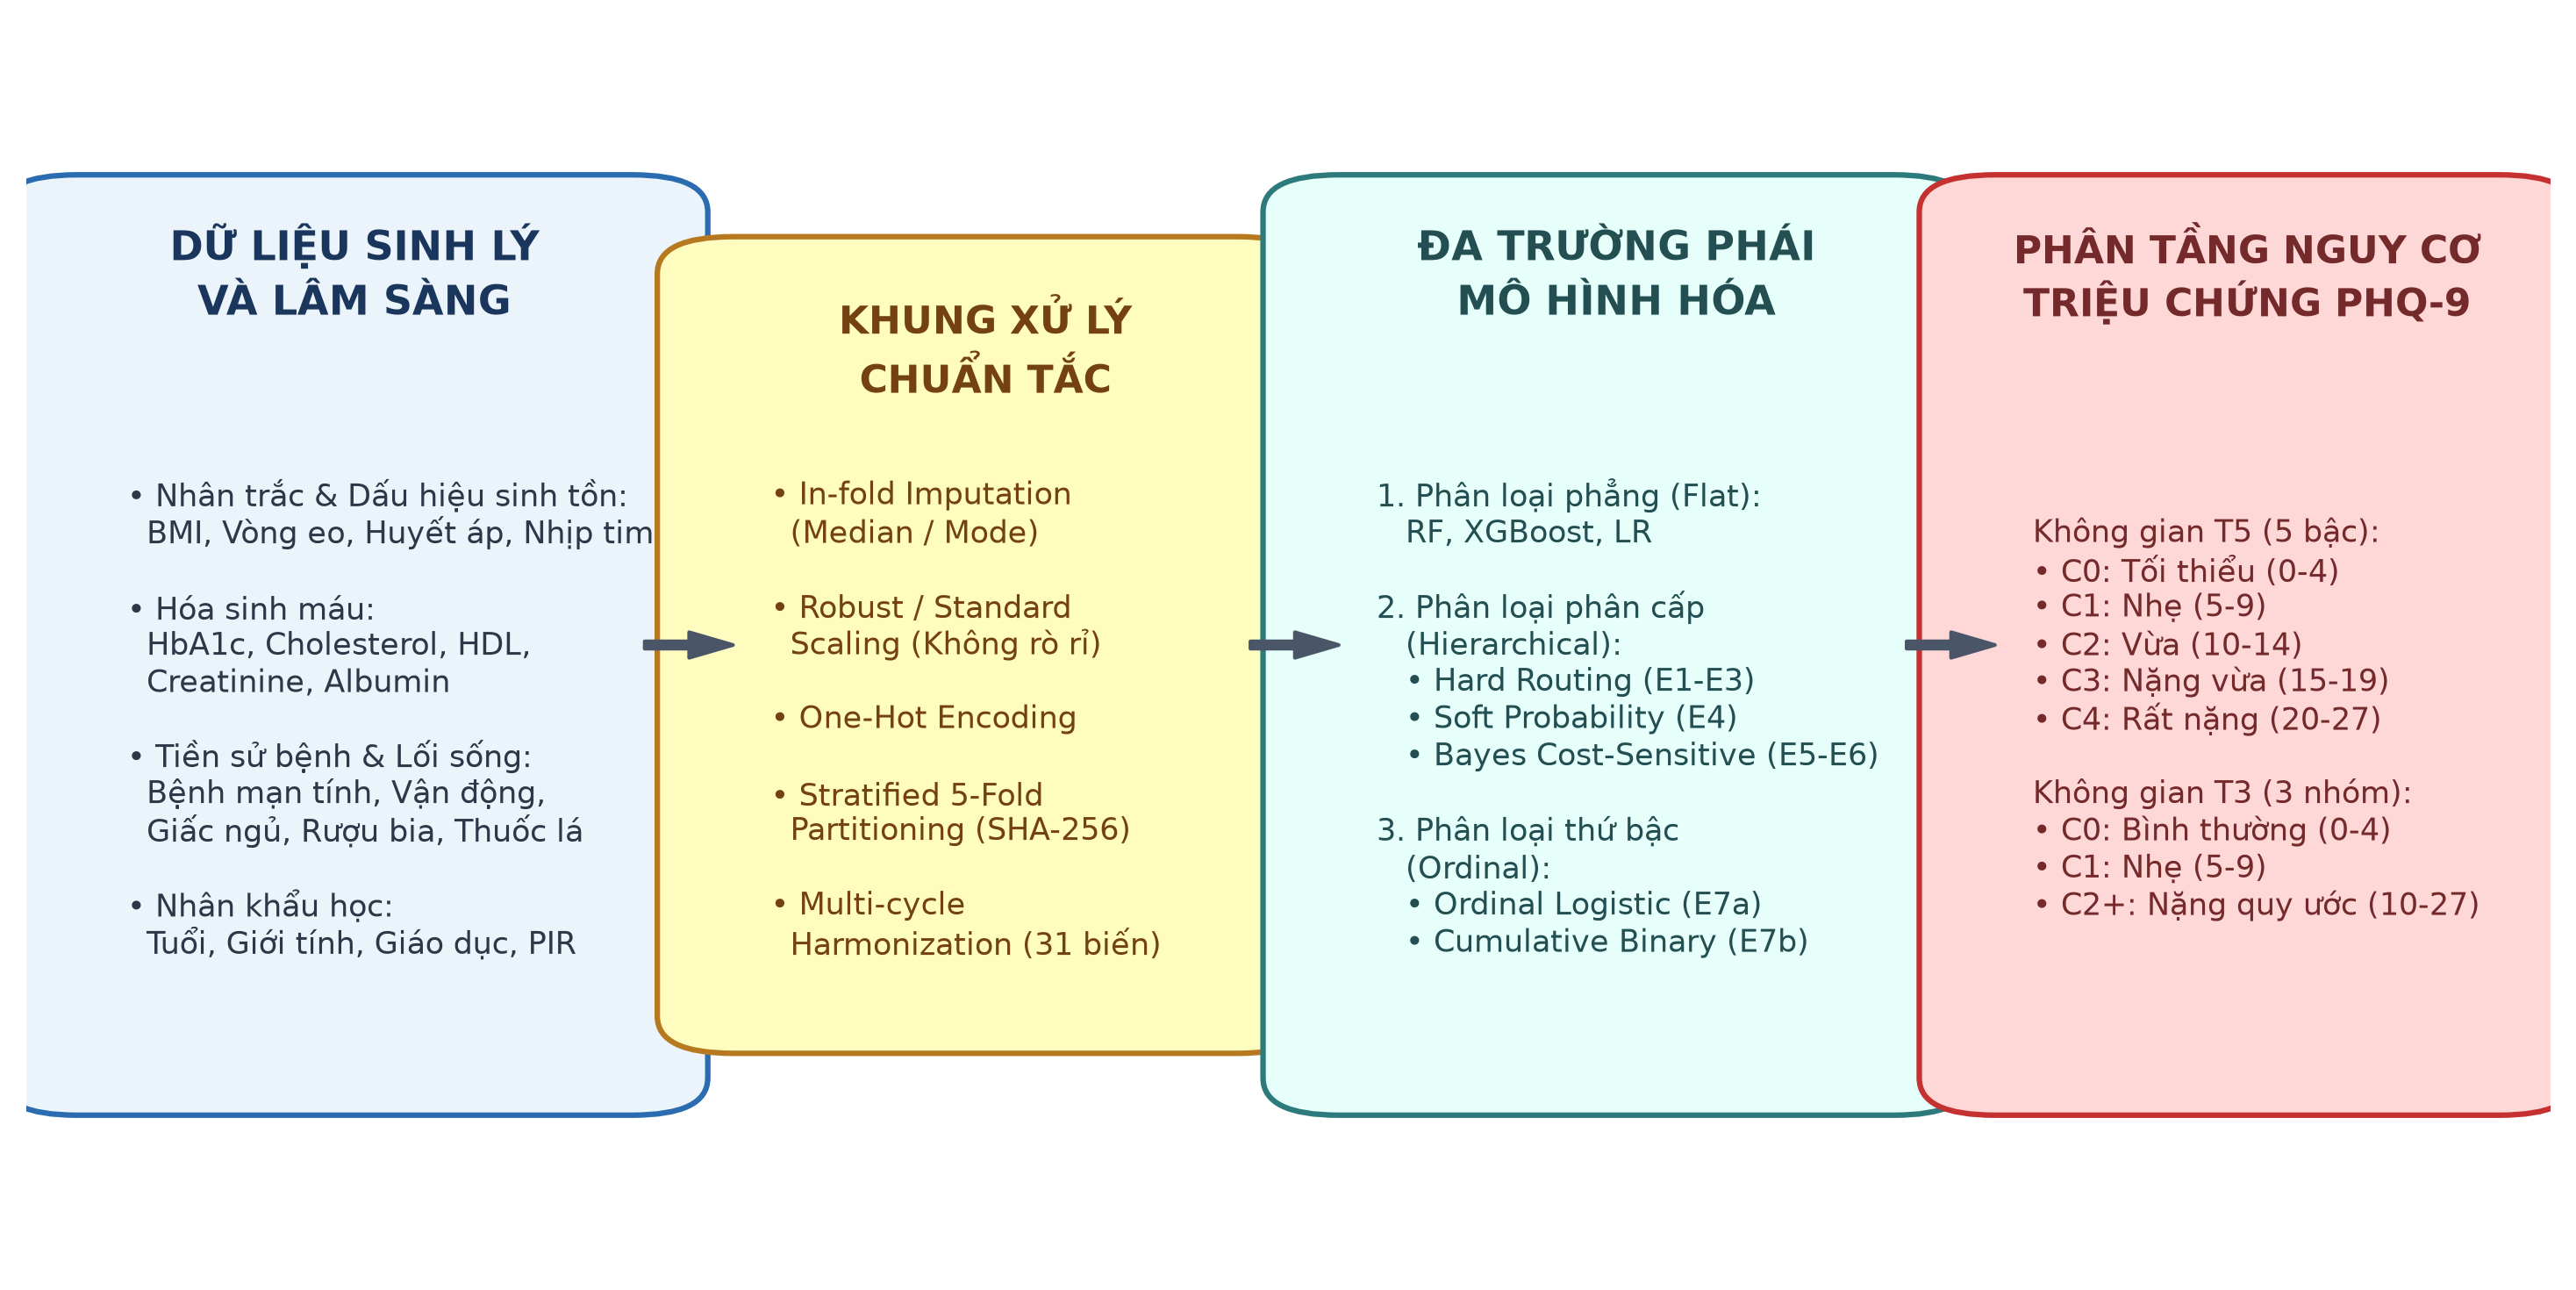
\includegraphics[width=\textwidth]{figures/fig1_problem_formulation.png}
\label{fig:problem-formulation}
\end{figure}
\FloatBarrier

\textbf{Ràng buộc kỹ thuật bắt buộc (Zero Data Leakage):} Để bảo đảm tính khách quan và khả năng khái quát hóa y sinh thực chất, ma trận đặc trưng đầu vào $\mathbf{X}$ tuyệt đối không được chứa bất kỳ câu hỏi nào trong số 9 câu hỏi khảo sát DPQ. Toàn bộ các bước chuẩn hóa, điền khuyết (imputation) và mã hóa đặc trưng bắt buộc phải được học độc lập bên trong từng tập huấn luyện của kiểm định chéo (Cross-Validation fold) và chỉ được áp dụng lên tập kiểm tra.

\section{Mục tiêu và câu hỏi nghiên cứu}
\label{sec:muc-tieu-va-cau-hoi}

Mục tiêu tổng quát của đề tài là xây dựng một khung học máy thực nghiệm hoàn chỉnh, có khả năng tái lập và kiểm soát chặt chẽ, nhằm khảo sát và nâng cao hiệu năng dự đoán mức độ triệu chứng trầm cảm từ dữ liệu sinh lý đa chu kỳ NHANES. 

Để đạt được mục tiêu tổng quát, nghiên cứu tập trung giải quyết năm câu hỏi khoa học trọng tâm (Research Questions -- RQ):
\begin{itemize}
    \item \textbf{RQ1 (Đóng góp của các nhóm đặc trưng):} Những nhóm đặc trưng nào (trong số nhân trắc học, huyết áp, hóa sinh máu, huyết học, lối sống và nhân khẩu học) đóng góp thực chất nhất vào khả năng dự đoán mức độ PHQ-9, và sự kết hợp đa tầng đặc trưng có giúp cải thiện hiệu năng so với từng nhóm đơn lẻ không?
    \item \textbf{RQ2 (Quy luật suy giảm theo độ chi tiết nhãn):} Hiệu năng của các mô hình học máy thay đổi như thế nào khi độ chi tiết của nhãn mục tiêu tăng dần từ 2 lên 3, 4 và 5 mức độ? Bước chuyển dịch nào và ranh giới nhãn nào là nguyên nhân chính gây ra sự suy giảm hiệu năng lớn nhất?
    \item \textbf{RQ3 (Tác động của việc mở rộng dữ liệu đa chu kỳ):} Liệu việc mở rộng cỡ mẫu từ một chu kỳ đơn lẻ ($N = 5.054$) lên ba chu kỳ gộp ($N = 14.581$) với không gian đặc trưng hài hòa có thể khắc phục được hiện tượng suy giảm hiệu năng ở các mức độ chi tiết hay không?
    \item \textbf{RQ4 (Hiệu quả của phân loại phân cấp):} Kiến trúc phân loại phân cấp hai giai đoạn (Hierarchical Classification) có cải thiện được hiệu năng phân loại trên không gian 3 lớp ($T_3$) so với phân loại phẳng truyền thống (Flat Classification) hay không, và cơ chế định tuyến cứng (Hard Routing) gây ra những hệ quả nào đối với sự lan truyền sai số (Error Propagation)?
    \item \textbf{RQ5 (Khả năng của Soft, Cost-Sensitive và Ordinal Classification):} Việc chuyển đổi từ định tuyến cứng sang định tuyến mềm (Soft Probability Fusion), tối ưu hóa rủi ro Bayes theo ma trận chi phí (Cost-Sensitive Learning) và mô hình hóa trực tiếp quan hệ thứ bậc (Ordinal Classification) giải quyết được những mâu thuẫn nào giữa Macro-F1, Balanced Accuracy, Class MAE và tỷ lệ bỏ sót ca bệnh nặng?
\end{itemize}

\section{Phạm vi và giới hạn nghiên cứu}
\label{sec:pham-vi-nghien-cuu}

Để định hình rõ ranh giới học thuật của đề tài, các giới hạn nghiên cứu được xác định minh bạch như sau:
\begin{enumerate}
    \item \textbf{Miền dữ liệu:} Nghiên cứu giới hạn trên tập dữ liệu khảo sát cắt ngang dạng bảng của NHANES (Hoa Kỳ) ở các chu kỳ 2011--2012, 2013--2014 và 2015--2016, áp dụng cho đối tượng người trưởng thành từ 20 tuổi trở lên có đầy đủ 9 mục khảo sát PHQ-9 hợp lệ.
    \item \textbf{Bản chất tín hiệu:} Đề tài chỉ sử dụng các đặc trưng sinh lý và cận lâm sàng dạng bảng được trích xuất từ hồ sơ khám sức khỏe định kỳ. Nghiên cứu \textbf{không sử dụng tín hiệu chuỗi thời gian thô} như điện tâm đồ (ECG) liên tục hay điện não đồ (EEG).
    \item \textbf{Tính chất bài toán:} Đề tài tập trung vào bài toán lượng giá mức độ triệu chứng trầm cảm tự báo cáo (symptom severity prediction) trong nghiên cứu dịch tễ, \textbf{không phải là hệ thống chẩn đoán bệnh học lâm sàng tự động}. Kết quả đầu ra là điểm số và nhãn nhóm nguy cơ, không thay thế quy trình thăm khám tâm thần chuyên sâu.
    \item \textbf{Đóng góp thuật toán:} Nghiên cứu tập trung vào thiết kế kiến trúc hệ thống, tích hợp các phương pháp phân loại phân cấp, quyết định nhạy chi phí và phân loại thứ bậc để giải quyết bài toán mất cân bằng lớp và chồng lấn đặc trưng trong dữ liệu y tế thực tế, đảm bảo tính chặt chẽ về mặt phương pháp luận.
\end{enumerate}

\section{Phương pháp tiếp cận và đóng góp của đề tài}
\label{sec:dong-gop-nghien-cuu}

Nghiên cứu tiếp cận theo quy trình 5 bước chặt chẽ: (1) Hài hòa hóa dữ liệu đa chu kỳ và cô lập in-fold; (2) Phân tích đóng góp đặc trưng $F_1 \to F_4$; (3) Đánh giá trần hiệu năng theo độ phân giải nhãn $T_2 \to T_5$; (4) Khảo sát các kiến trúc phân cấp cứng, phân cấp mềm và thứ bậc trên $T_3$; (5) Kiểm định ngoại suy độc lập theo thời gian trên chu kỳ tương lai NHANES 2015--2016.

Những đóng góp học thuật và thực tiễn chính của đề tài bao gồm:
\begin{enumerate}
    \item \textbf{Khảo sát thực nghiệm có kiểm soát chặt chẽ về trần hiệu năng:} Xác lập đường cơ sở thực nghiệm vững chắc trên 4 họ thuật toán qua 4 không gian đặc trưng lũy tiến ($F_1 \to F_4$), chỉ ra rằng việc bổ sung tiền sử bệnh lý ($F_2$) và lối sống/nhân khẩu ($F_3, F_4$) nâng Macro-F1 từ 0.1900 lên 0.2707, song vẫn chạm ngưỡng trần do tính chất gián tiếp của tín hiệu sinh lý.
    \item \textbf{Lượng hóa quy luật suy thoái theo độ chi tiết nhãn và phân tích nguyên nhân sinh lý:} Chứng minh quy luật sụt giảm hiệu năng mạnh khi tăng số lớp từ $T_2$ (Macro-F1 = 0.6639) xuống $T_5$ (Macro-F1 = 0.2630), đồng thời phân tích hình học bằng PCA và tương quan sinh hóa nhằm khẳng định nguyên nhân cốt lõi là do sự chồng lấn phân phối dày đặc giữa lớp bình thường ($C_0$) và triệu chứng nhẹ ($C_1$).
    \item \textbf{Phát hiện điểm nghẽn lan truyền sai số và đề xuất giải pháp mềm nhạy chi phí:} Phân tích cấu trúc phân loại phân cấp cứng hai giai đoạn ($E_1 \to E_3$), vạch trần điểm nghẽn nghiêm trọng khi loại bỏ nhầm 120 ca nặng quy ước ($C_2^+$) ngay từ giai đoạn sàng lọc đầu tiên; từ đó đề xuất mô hình phân cấp mềm kết hợp ma trận chi phí Bayes ($E_6b$) giúp giảm mạnh số ca bỏ sót xuống còn 31 ca (giảm 74.2\%).
    \item \textbf{Khảo sát mô hình phân loại thứ bậc và kiểm định độc lập theo dòng thời gian:} Đánh giá toàn diện mô hình Hồi quy Logistic thứ bậc (OLR) và Phân loại nhị phân tích lũy (CBC), chứng minh OLR cân bằng đạt Balanced Accuracy cao nhất (0.5151) và duy trì sự ổn định vượt trội khi kiểm định ngoại suy trên tập dữ liệu tương lai độc lập NHANES 2015--2016 ($N = 4.888$, Balanced Accuracy = 0.5073).
\end{enumerate}

\section{Cấu trúc báo cáo}
\label{sec:bo-cuc-khoa-luan}

Báo cáo dự án khoa học được cấu trúc thành 5 chương chính như sau:
\begin{itemize}
    \item \textbf{Chương 1: Giới thiệu} -- Trình bày bối cảnh nghiên cứu, phát biểu bài toán toán học, mục tiêu, 5 câu hỏi nghiên cứu, phạm vi và các đóng góp chính.
    \item \textbf{Chương 2: Cơ sở lý thuyết và các nghiên cứu liên quan} -- Làm rõ thang đo PHQ-9 và cơ sở sinh lý học, đặc thù mất cân bằng lớp và chồng lấn đặc trưng trong dữ liệu y tế dạng bảng, các trường phái mô hình hóa (phẳng, phân cấp, thứ bậc) và tổng quan các công trình tiền nhiệm.
    \item \textbf{Chương 3: Dữ liệu và phương pháp nghiên cứu} -- Trình bày kiến trúc hệ thống 7 module, nguồn dữ liệu và giao thức hài hòa hóa, hệ thống đặc trưng lũy tiến, các thiết kế kiến trúc phân loại ($E_0 \to E_7$) và quy trình kiểm thử nghiêm ngặt.
    \item \textbf{Chương 4: Thực nghiệm và thảo luận} -- Báo cáo chi tiết môi trường thực nghiệm, kết quả Feature Ablation, tối ưu hóa siêu tham số, phân tích độ chi tiết nhãn, thực nghiệm đa chu kỳ, khảo sát $E_0 \to E_7$, phân tích đánh đổi lâm sàng và kiểm định theo dòng thời gian.
    \item \textbf{Chương 5: Kết luận và hướng phát triển} -- Tổng kết toàn bộ kết quả, đánh giá các hạn chế thực tế của dữ liệu và đề xuất các hướng mở rộng tiếp theo.
\end{itemize}

